%---------------------------------- Problem definition -------------------------------
\begin{frame}{Problem Definition}
    This problem can be characterized the optimization of an \large\textbf{expensive, mixed-variable, noisy, blackbox} function.

    \begin{columns}
    
        \begin{column}[t]{0.5\textwidth}
        \begin{block}{Problem Formulation}
            The HPO problem can be defined as 
            \begin{equation}
               \eta^* \in \arg\min_{\eta \in \mathcal{H}} \mathcal{F}(\eta) 
            \end{equation}

        \end{block}

        \begin{block}{Search Space $\mathcal{H}$}
            $\mathcal{H}$ is the set of all values the solution tuple $\eta$ can take. This stage includes method to handle the mixed-variables aspect of the problems.   
        \end{block}
        \end{column}
        
        \begin{column}[t]{0.5\textwidth}

    
        \begin{block}{Search Strategy}
            With $\eta_i$ all the tested solutions, the search strategy is the method used to define the next solution $\eta_{next}$ to evaluate. 
        \end{block}

        \begin{block}{Perfomance Evaluation Strategy}
            $\mathcal{F}$ represent the objective function, how the function is implemented. Also includes method like multi-fidelity that affect the fidelity of the evaluation.
        \end{block}

        \end{column}
         
  \end{columns}
\end{frame}


%------------------------------------ Search Space ---------------------------
\begin{frame}{Search Space}

    The search space is composed of variables of different type.

    \begin{block}{Hyper-parameters}
    
        \begin{table}[h!]
            \centering
            \begin{tabular}{|c|c|c|c|}
                \hline
                \multirow{2}{*}{\textbf{Hyper-parameter}} & \multicolumn{2}{|c|}{\textbf{Optimization range}} & \multirow{2}{*}{\textbf{Conversion}} \\
                \cline{2-3}
                 & \textbf{Lower Bound} & \textbf{Upper Bound} &  \\
                \hline
                \textbf{Learning Rate} & $-10$ & $-1$ & $f(x) = 10^{x}$ \\
                \hline
                \textbf{LoRA Rank} & 2 & 512 & $f(x) = \text{round}(x)$ \\
                \hline
                \textbf{LoRA scale ($\alpha$)} & 1 & 64 & $f(x) = \text{round}(x)$ \\
                \hline
                \textbf{LoRA Dropout} & 0 & 0.5 & $f(x) = x$ \\
                \hline
                \textbf{Weight Decay} & $-5$ & $-1$ & $f(x) = 10^{x}$  \\
                \hline
            \end{tabular}
            \caption{Summary of Hyperparameter Search Space}
            \label{tab:hyperparam_table}
        \end{table}
        
    \end{block}
    
    Conversion and naming convention is taken from LitGPT framework.
\end{frame}


%---------------------------------- Search Strategy  -------------------------------
\begin{frame}[allowframebreaks]{Search Strategy}
    The search strategy of an optimization problem can be seen as a balance between the exploration, i.e. going to unexplored regions, and exploitation, i.e. going close to promising areas. Here are the fields of optimization to tackle HPO problems.

\end{frame}

\begin{frame}{Exploratory Method}
    \begin{columns}
        % Left Column (Text)
        \begin{column}{0.5\textwidth}
            \begin{block}{Grid Search and Random Search}
                These 2 methods are the simplest way possible of exploring the search space, without exploiting the acquired knowledge. Useful to assess the pertinence of the optimization algorithm.        
            \end{block}
        \end{column}

        % Right Column (Image)
        \begin{column}{0.5\textwidth}
            \begin{figure}
                \centering
                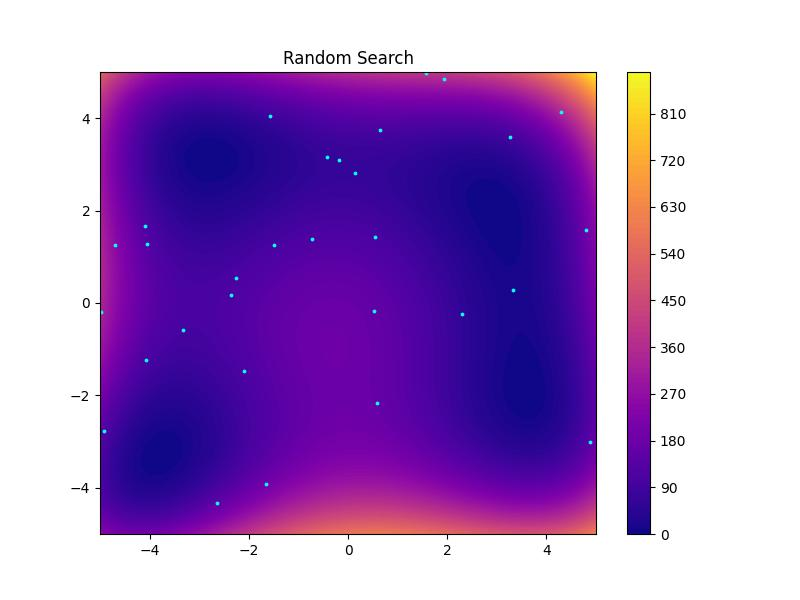
\includegraphics[width=\linewidth]{imgs/plots/random_search.jpg}
                \caption{Random Search}
            \end{figure}
        \end{column}
    \end{columns}
\end{frame}

\begin{frame}{Meta-heuristics}

    \begin{block}{Meta-heuristics}
        Meta-heuristics are mostly algorithms inspired by nature, divided in 2 approachs : population evolution or individual evolution. For the first one, methods like Genetic Algorithm (GA) allow the fitting of the population to a problem, with evolutionnary operators like crossover, mutation or selection. For the second one, like Intensive Local Search (ILS), the methods iterate through the search space with only one solution by iteration. \\
        These methods aren't fit to HPO problems applied to LLM, due of their needs of numerous evaluations, begin computationally prohibitive. 
        
    \end{block}
    
\end{frame}

    
\begin{frame}{Partition Based Optimization}

    \begin{columns}
        % Left Column (Text)
        \begin{column}{0.5\textwidth}
            \begin{block}{Partition Based Optimization}
                Sets of methods that apply partition to the search space, to favor (partition again) or penalize (discard region) these partitions.  E.g.: DIRECT\cite{jones1993direct}, Fractals\cite{firmin:hal-04474444}, SOO\cite{munos2011soo}\\

                Useful for parallelization abilities
            \end{block}
        \end{column}

        % Right Column (Image)
        \begin{column}{0.5\textwidth}
            \begin{figure}
                \centering
                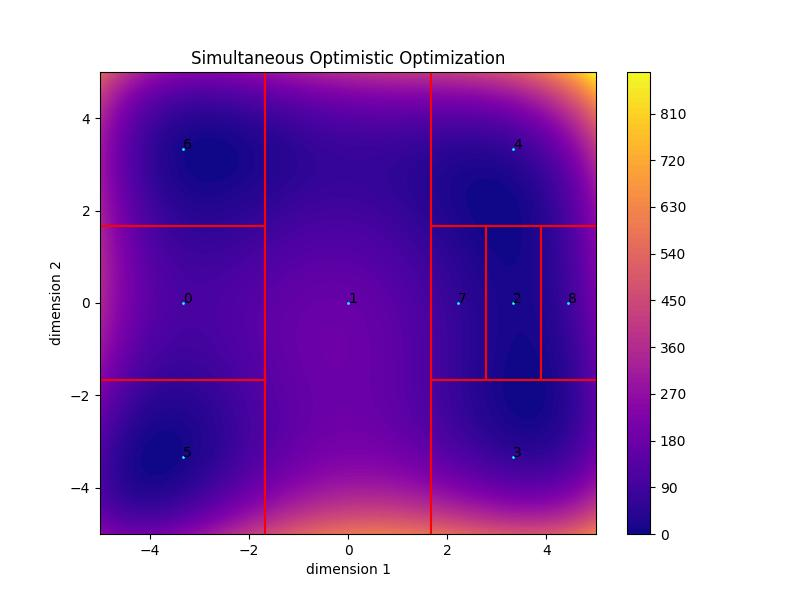
\includegraphics[width=\linewidth]{imgs/plots/soo.jpg}
                \caption{SOO}
            \end{figure}
        \end{column}
    \end{columns}

\end{frame}


\begin{frame}{Surrogate-Model Based Optimization (SMBO)}

    \begin{columns}
        % Left Column (Text)
        \begin{column}{0.5\textwidth}
                Methods based on creating a \textbf{surrogate} model of the objective function, using the knowledge from already evaluated solutions. The acquisition function, i.e. the function of the surrogate model, is used to balance exploration and exploitation. \\
                
                E.g.: Bayesian Modeling, Gaussian Process (GP), Tree Parzen Estimator (TPE).\\
        \end{column}

        % Right Column (Image)
        \begin{column}{0.5\textwidth}
            \begin{figure}
                \centering
                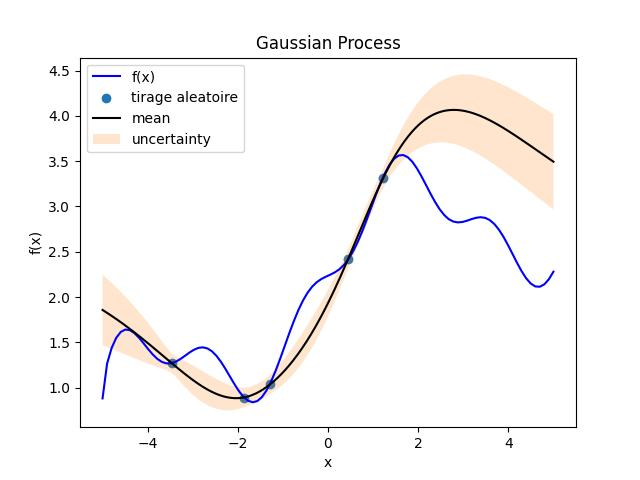
\includegraphics[width=\linewidth]{imgs/plots/gaussian_process.jpg}
                \caption{Gaussian Process}
            \end{figure}
        \end{column}
    \end{columns}

\end{frame}

\begin{frame}{Partition and Surrogate-Model based optimization : the hybridation}

    \begin{columns}
        % Left Column (Text)
        \begin{column}{0.5\textwidth}
        The partition based methods are by nature parallel, by the generation of a tree-search of possible solutions. The SMBO achieve to reduce the number of evaluation by using an acquisition function to discard or favor a possible solution. The hybridation would result in a parallelization-able Bayesian modeling, allowing to extract the best of the two fields. \\
           
        \end{column}

        % Right Column (Image)
        \begin{column}{0.5\textwidth}
            \begin{figure}
                \centering
                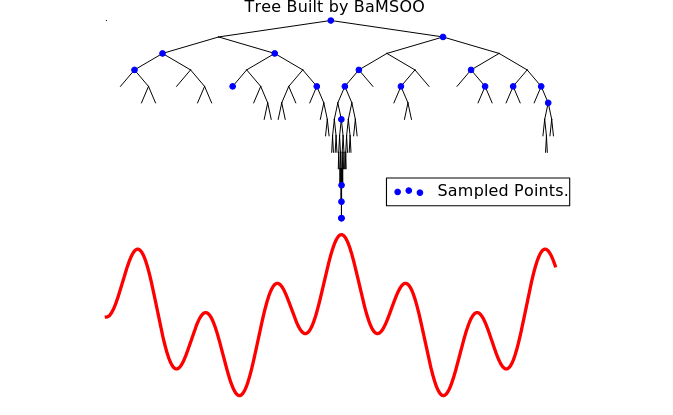
\includegraphics[width=\linewidth]{imgs/bamsoo.png}
                \caption{BaMSOO \cite{wang2014bamsoo}}
            \end{figure}
        \end{column}
    \end{columns}

\end{frame}

%---------------------------------- Performance Evaluation Strategy -------------------------------

\begin{frame}{Performance Evaluation Strategy}
    \begin{block}{Evaluation context}
    In this part, there are many options, like the number of epochs (if not an hyperparameters), the precision of the model, the datasets of training or evaluation. 
        
    \end{block}
    \begin{block}{Objective function}
        For this problem, there are 2 ways to evaluate a solution : 
        \begin{itemize}
            \item Loss (validation or testing) : the loss is computed through the training, and we can keep a small part of the datasets unused to use it the evaluate the model. Cons : dataset dependant, difficult to put in global context
            \item \textbf{Benchmark dataset (GLUE\cite{wang2018glue}, MMLU\cite{hendrycks2021mmlu})} : the accuracy on a literature benchmark dataset can be used to evaluate the training. It's interesting, since it's a good measure of generalization, since the model has not read this type of questions. Warning : the benchmark used during the optimization can't be used as a final testing. 
        \end{itemize}

        Multi-fidelity approaches can be used to reduce the cost of evaluation in earlier steps. Algorithms like Bayesian Optimization and HyperBand (BOHB\cite{DBLP:journals/corr/abs-1807-01774}) achieve cost-efficient optimization by reducing the part of the datasets in early stages.
    \end{block}
    
\end{frame}